 \documentclass[5]{article}
\usepackage[utf8]{inputenc}
\usepackage{hyperref} 

\usepackage[T1]{fontenc}
\usepackage[polish]{babel}

\title{Laboratorium 5}
\author{Piotr Witek}
\date{21 kwietnia 2021}

\usepackage{natbib}
\usepackage{graphicx}
\usepackage{geometry}
\usepackage{tabularx}
\usepackage{array}
\usepackage{amsmath}

\begin{document}

\newgeometry{tmargin=2cm, bmargin=2cm, lmargin=2.5cm, rmargin=2.5cm}

\maketitle


\section{Mamy równanie: $f(x) = x^2 - 2 = 0$}

\textbf{(a) zakładając że mamy punkt początkowy x0 = 1, jaką wartość x1 dostaniemy,
jeśli używamy metody Newtona ?}
\newline


Wzór iteracyjny metody Newtona ma postać:
$$x_{k+1}=x_{k}-\frac{f\left(x_{k}\right)}{f^{\prime}\left(x_{k}\right)}$$

Obliczamy  $f\left(x_{0}\right)$ i  $f^{\prime}\left(x_{0}\right)$:
$$
\begin{array}{l}
f\left(x_{0}\right)=f(1)=1^{2}-2=-1 \\
f^{\prime}\left(x_{0}\right)=f^{\prime}(1)=\left.2 x\right|_{x=1}=2
\end{array}
$$
\hspace{4mm} Podstawiając do wzoru otrzymujemy:
$$
x_{1}=x_{0}-\frac{f\left(x_{0}\right)}{f^{\prime}\left(x_{0}\right)}=1-\frac{-1}{2}=1.5
$$

\vspace{5mm}

\textbf{(b) zakładając że mamy $ x_0 = 1$ i $x_1 = 2$ jako punkty początkowe, jaka będzie wartość x2, jeśli używamy metody siecznych do tego samego problemu?}
\newline

Metoda siecznych polega na prowadzeniu funkcji liniowych przechodzących przez dwa punkty $a$ i $b$ dla których szukana funkcja ma wartości o przeciwnych znakach, znalezieniu miejsca zerowego $c$ tej funkcji liniowej i stworzeniu ciągu, liczb takiego, że $x_{0}=a, x_{1}=b, x_{n}$ - miejsce zerowe funkcji liniowej przechodzącej przez punkty $\left(x_{n-1}, f\left(x_{n-1}\right)\right)$ i $\left(x_{n-2}, f\left(x_{n-2}\right)\right)$ Metodę tę powtarzamy do momentu uzyskania satysfakcjonującego nas przybliżenia funkcji.

Zgodnie $\mathrm{z}$ powyższą definicją $x_{2}$ będzie to miejsce zerowe funkcji liniowej przechodzącej przez punkty $(a, f(a)) \mathrm{i}(b, f(b))$ 

\newline
Równanie prostej przechodzącej przez punkty: $(a, f(a))$ i $(b, f(b))$ jest postaci:
$$
y=\frac{f(b)-f(a)}{b-a}(x-b)+f(b)
$$
Szukamy takiego $\mathrm{x}$ dla którego: $y=0$


$$0=\frac{f(b)-f(a)}{b-a}\left(x_{2}-b\right)+f(b)$$
$$\frac{f(b)-f(a)}{b-a} x_{2}=\frac{f(b)-f(a)}{b-a} b-f(b)$$
$$x_{2}=b-\frac{b f(b)-a f(b)}{f(b)-f(a)}=\frac{b f(b)-b f(a)}{f(b)-f(a)}-\frac{b f(b)-a f(b)}{f(b)-f(a)}=\frac{a f(b)-b f(a)}{f(b)-f(a)} $$
$$x_{2}=\frac{1 * f(2)-2 * f(1)}{f(2)-f(1)}=\frac{1 *\left(2^{2}-2\right)-2 *\left(1^{2}-2\right)}{\left(2^{2}-2\right)-\left(1^{2}-2\right)}=\frac{2+2}{2+1}=2.33333 \ldots $$





\section{Napisz iteracje wg metody Newtona do rozwiązywania każdego z następujących równań nieliniowych:}

\textbf{(a) $x^3 - 2x - 5 = 0$} \newline

Musimy poznać przebieg funkcji, aby w przybliżeniu określić granice przedziału zawierającego dany pierwiastek. W tym celu został wygenerowany wykres:

\begin{center}
    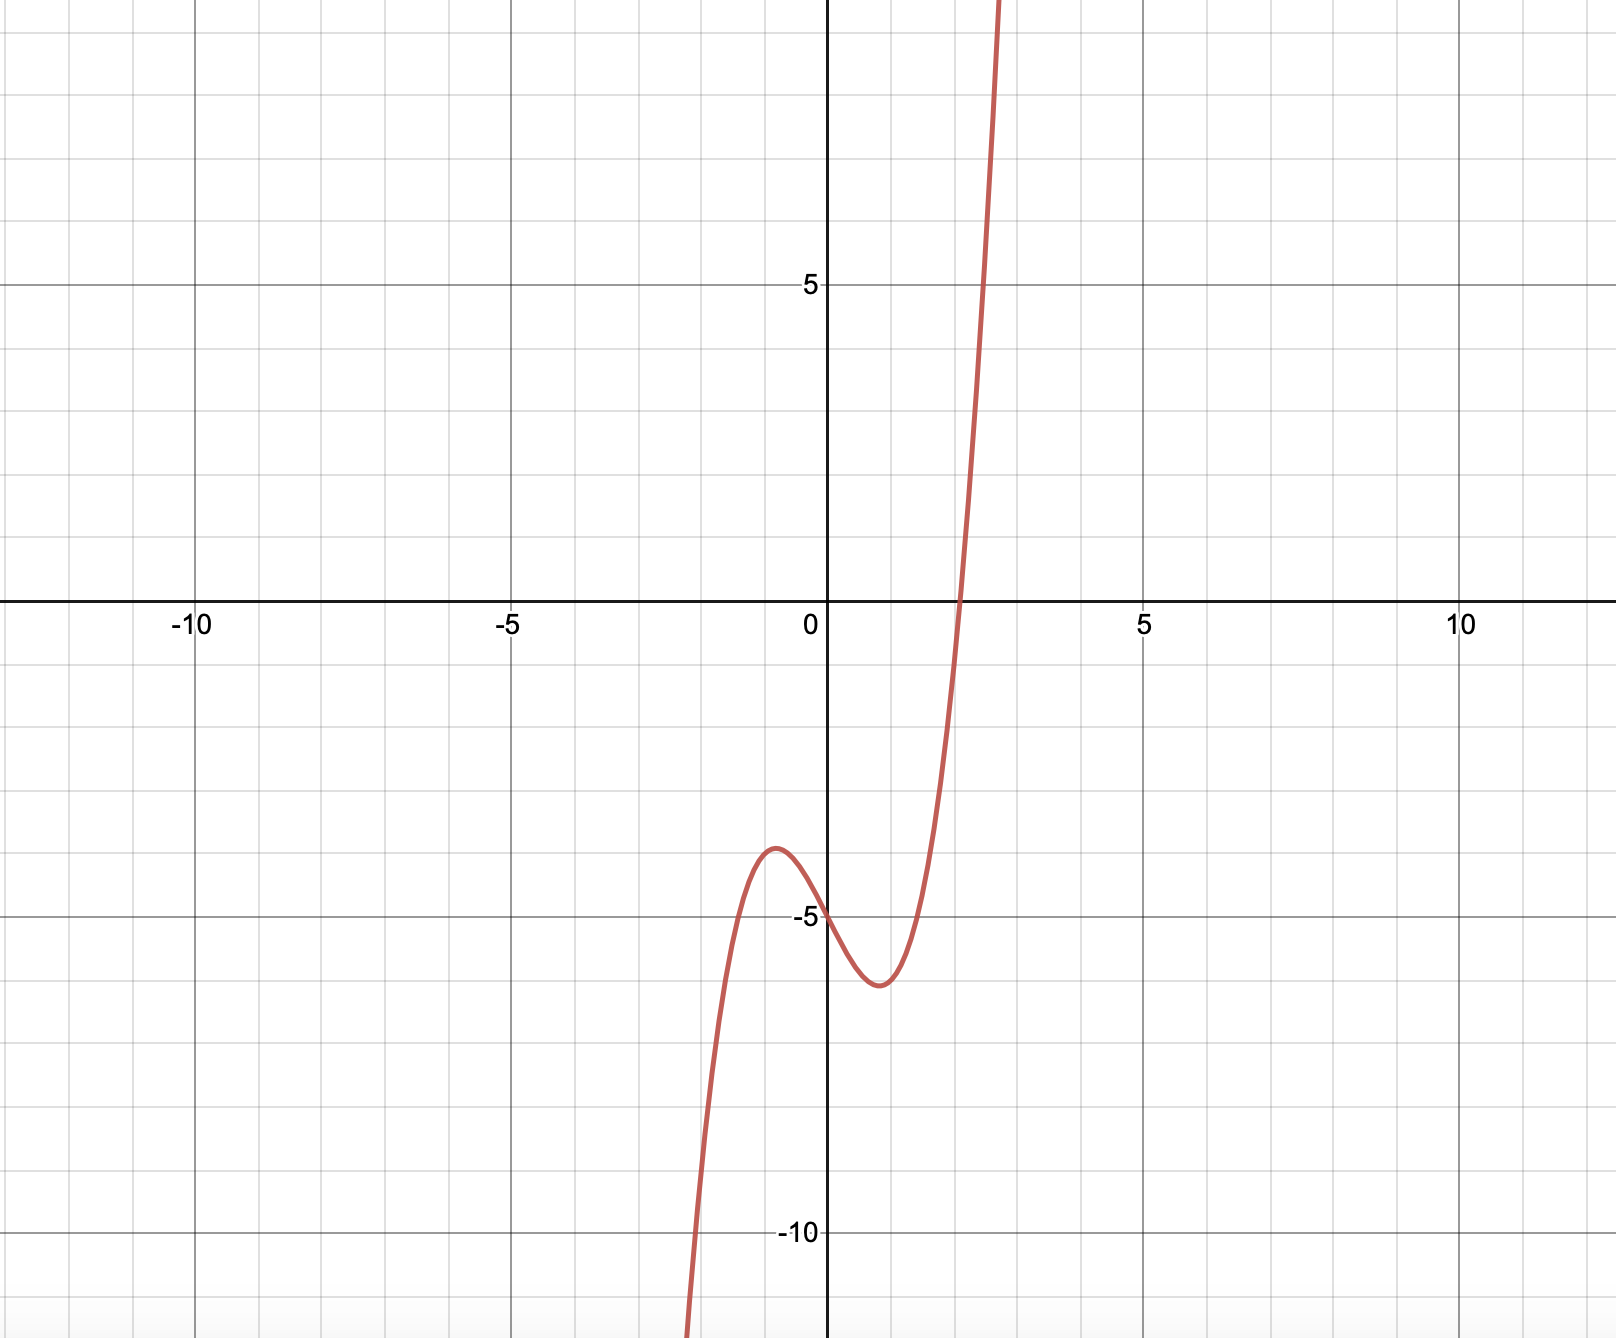
\includegraphics[scale=0.4]{lab5_1.png} \par
    \vspace{3mm}
    
\end{center}

\hfil{Rysunek 1: Wykres funkcji $f(x) = x^3 - 2x - 5$} \par

\vspace{5mm}

Miejsce zerowe znajduje się w przedziale [1,3] i jest to jedyne miejsce zerowe w tym przedziale więc zostało spełnione założenie pierwsze metody Newtona dla funkcji f. 

\vspace{5mm}
Sprawdzamy więc warunek $f(a)*f(b)<0$:
$$ f(1) = 1 - 2 - 5 = -6 < 0$$
$$ f(3) = 27 - 6 - 5 = 16 > 0$$

\vspace{3mm}
Widać że warunek $f(a)*f(b)<0$ został spełniony.
\vspace{5mm}

Musimy jeszcze sprawdzić znak wyrażenia $f'(x)*f''(x)$:

$$f'(x) = 3x^2 - 2, f'(1) = 1, f'(3) = 25$$
$$f''(x) = 6x, f''(1) = 6, f''(3) = 18$$
\newline

Widać że znak jest zawsze dodatni, więc wybieramy punkt startowy: $x_0 = b = 3$

Sprawdzam warunek zbieżności dla $x=3:\left|\frac{f(x) \cdot f^{\prime \prime}(x)}{\left(f^{\prime}(x)\right)^{2}}\right|<1 \Leftrightarrow\left|\frac{f(3) \cdot f^{\prime \prime}(3)}{\left(f^{\prime}(3)\right)^{2}}\right|<1 \Leftrightarrow 0.13328<1$.

\vspace{7mm}

$
\begin{array}{ll}
x_{0}=3 \\
x_{1}=3-\frac{f(3)}{f^{\prime}(3)} \approx 2.36  & \quad\left|x_{1}-x_{0}\right| \approx 0.232803 \\
x_{2}=2.36-\frac{f(2.36)}{f^{\prime}(2.36)} \approx 2.1272 &\quad\left|x_{2}-x_{1}\right| \approx 0.0320606 \\
x_{3}=2.1272-\frac{f(2.1272)}{f^{\prime}(2.1272)} \approx 2.09514  &\quad\left|x_{3}-x_{2}\right| \approx 0.00058447 \\
x_{4}=2.09514-\frac{f(2.09514)}{f^{\prime}(2.09514)} \approx 2.09455  &\quad\left|x_{4}-x_{3}\right| \approx 2 \cdot 10^{-7}<\varepsilon
\end{array}
$

\vspace{3mm}
Dla $x_{4}$ warunek został spełniony. Zatem można uznać, że dla określonej dokładności $\varepsilon=10^{-6}$ wynik $x_{4} \approx 2.09455$ jest szukanym miejscem zerowym funkcji.


\vspace{5mm}


\textbf{(b) $e^{-x} = x$} \newline

W celu okreslenia granic przedziału w którym znajduje się pierwiastek znowu musimy poznać wykres funkcji.

\begin{center}
    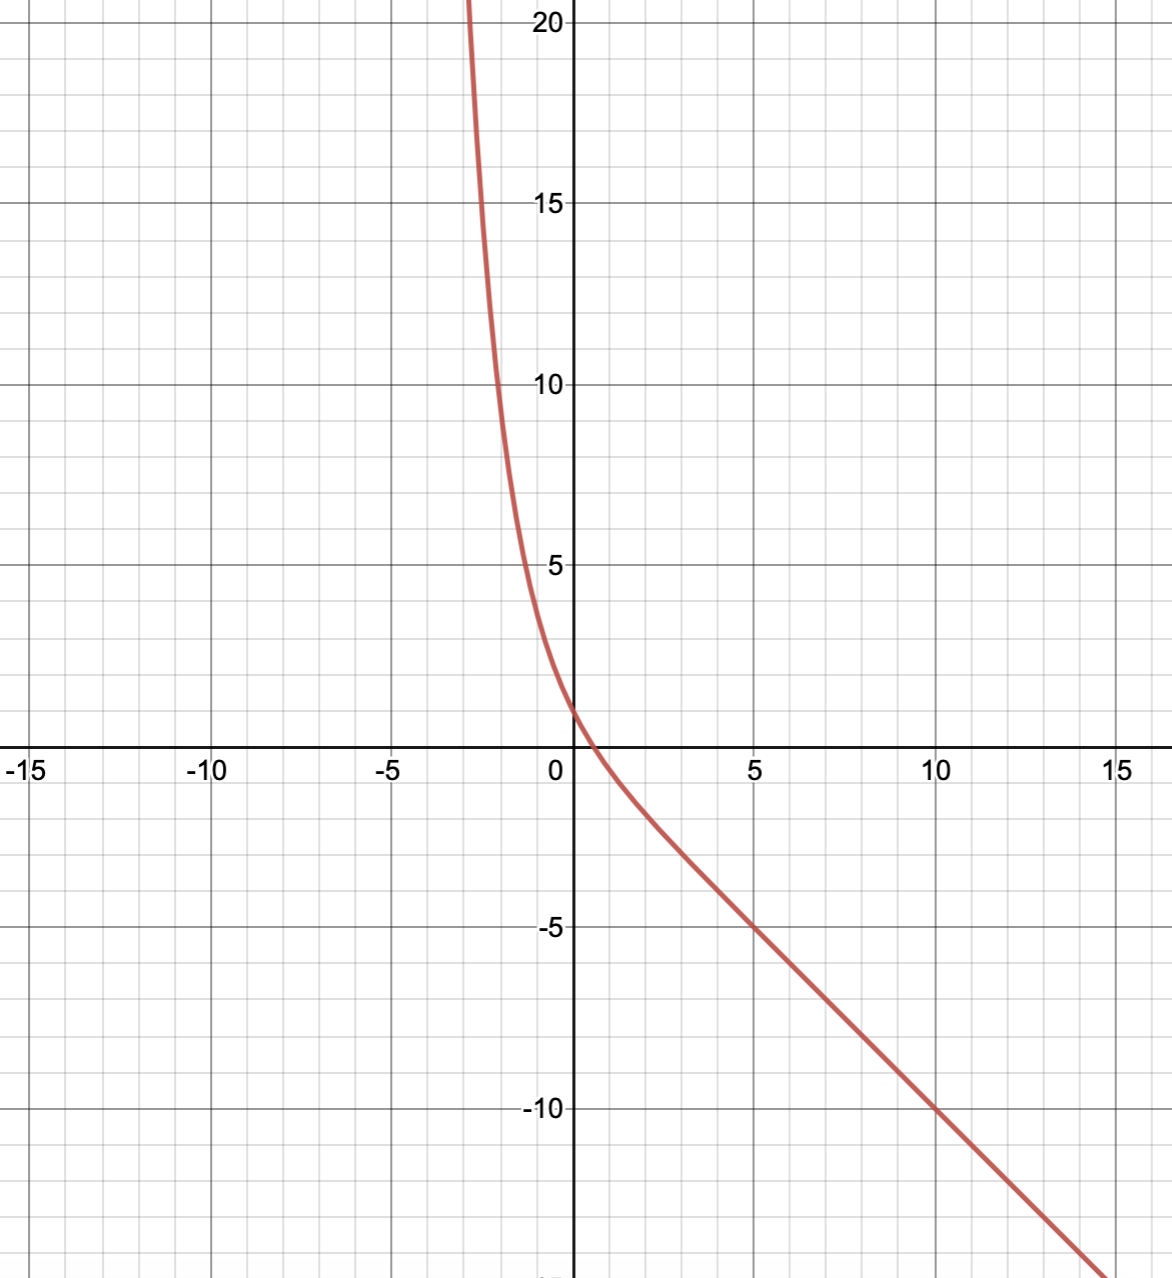
\includegraphics[scale=0.4]{lab5_2.png} \par
    \vspace{2mm}
    
\end{center}

\hfil{Rysunek 2: Wykres funkcji $f(x) = e^{-x} - x$} \par

\vspace{5mm}

 Możemy stwierdzić, że pierwiastek wystepuje $\mathrm{z}$ w przedziale $[-1,2]$. Sprawdźmy teraz warunek $f(a) \cdot f(b)<0$, gdzie $[\mathrm{a}, \mathrm{b}]$ to $[-1,2]$.
 
\vspace{1mm}


$$f(-1)=1+e \approx 3.71828$$
$$f(2)=-2+\frac{1}{e^{2}} \approx-1.86466$$

\vspace{2mm}

Warunek $f(-1) \cdot f(2) \approx-6.93335<0$ został spełniony więc w przyjętym przedziale pierwiastek na pewno występuje. Musimy sprawdzić jaki znak ma wyrażenie:  $f'(x)*f''(x)$ dla punktów brzegowych:

$$f^{\prime}(x)=-1-e^{-x}, f'(-1) = -3.718, f'(2) = -1.135$$
$$f^{\prime \prime}(x)=e^{-x}, f''(-1) = 2.718, f''(2) = 0.135$$

Zauważamy że znak wyrażenia jest zawsze ujemny więc wybieramy punkt startowy $x_{0}=a=-1$. Warunek stopu dobieramy jako $\varepsilon=10^{-6}$ i sprawdzamy warunek zbieżności dla $x=-1:\left|\frac{f(x) \cdot f^{\prime \prime}(x)}{\left(f^{\prime}(x)\right)^{2}}\right|<1 \Leftrightarrow\left|\frac{f(-1) \cdot f^{\prime \prime}(-1)}{\left(f^{\prime}(-1)\right)^{2}}\right|<1 \Leftrightarrow 0.731<1$.

$
\begin{array}{ll}
x_{0}=-1 \\
x_{1}=-1-\frac{f(-1)}{f^{\prime}(-1)} \approx 0 &\left|x_{1}-x_{0}\right| \approx 1 \\
x_{2}=0-\frac{f(0)}{f^{\prime}(0)} \approx 0.5 
&\left|x_{2}-x_{1}\right| \approx 0.5 \\ 
x_{3}=0.5-\frac{f(0.5)}{f^{\prime}(0.5)} \approx 0.56631
&\left|x_{3}-x_{2}\right| \approx 0.066311 \\
x_{4}=0.56631-\frac{f(0.56631)}{f^{\prime}(0.56631)} \approx 0.567143165 &\quad\left|x_{4}-x_{3}\right| \approx 0.000832162 \\
x_{5}=0.56714-\frac{f(0.56714)}{f^{\prime}(0.56714)} \approx 0.567143290 &\quad\left|x_{5}-x_{4}\right| \approx 1.25 \cdot 10^{-7}<\varepsilon
\end{array}
$

\vspace{2mm}

Dla $x_{5}$ warunek został spełniony. Zatem można uznać, że dla określonej dokładności $\varepsilon=10^{-6}$ wynik $x_{5} \approx 0.56714$ jest szukanym miejscem zerowym funkcji.

\vspace{5mm}

\textbf{(c) $x sin(x) = 1$}
\vspace{2mm}

Tutaj również warto spojrzeć na wykres: 

\begin{center}
    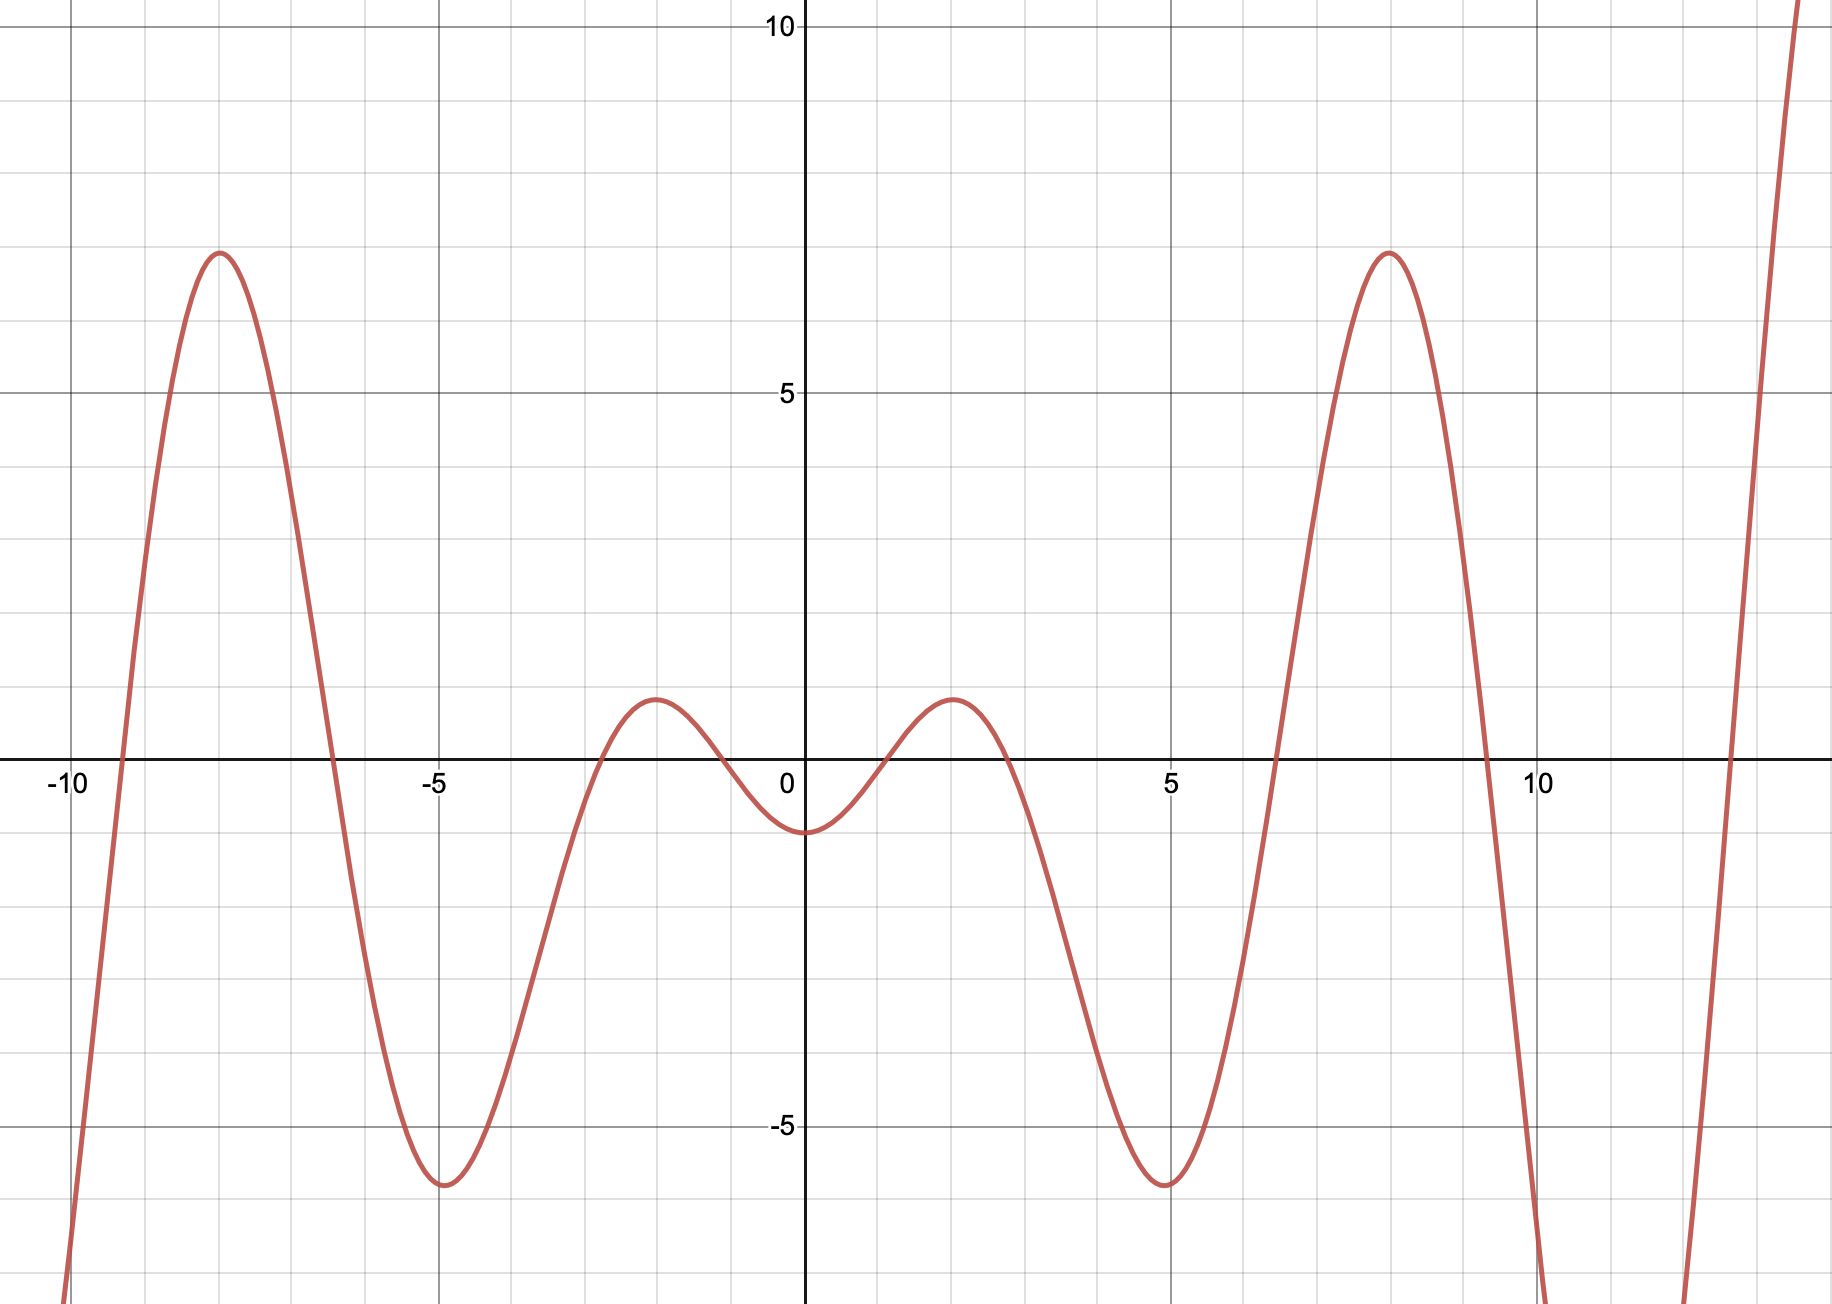
\includegraphics[scale=0.3]{lab5_31.png} \par
    \vspace{2mm}
    
\end{center}

\hfil{Rysunek 3: Wykres funkcji $f(x) = e^{-x} - x$} \par

% \begin{center}
%     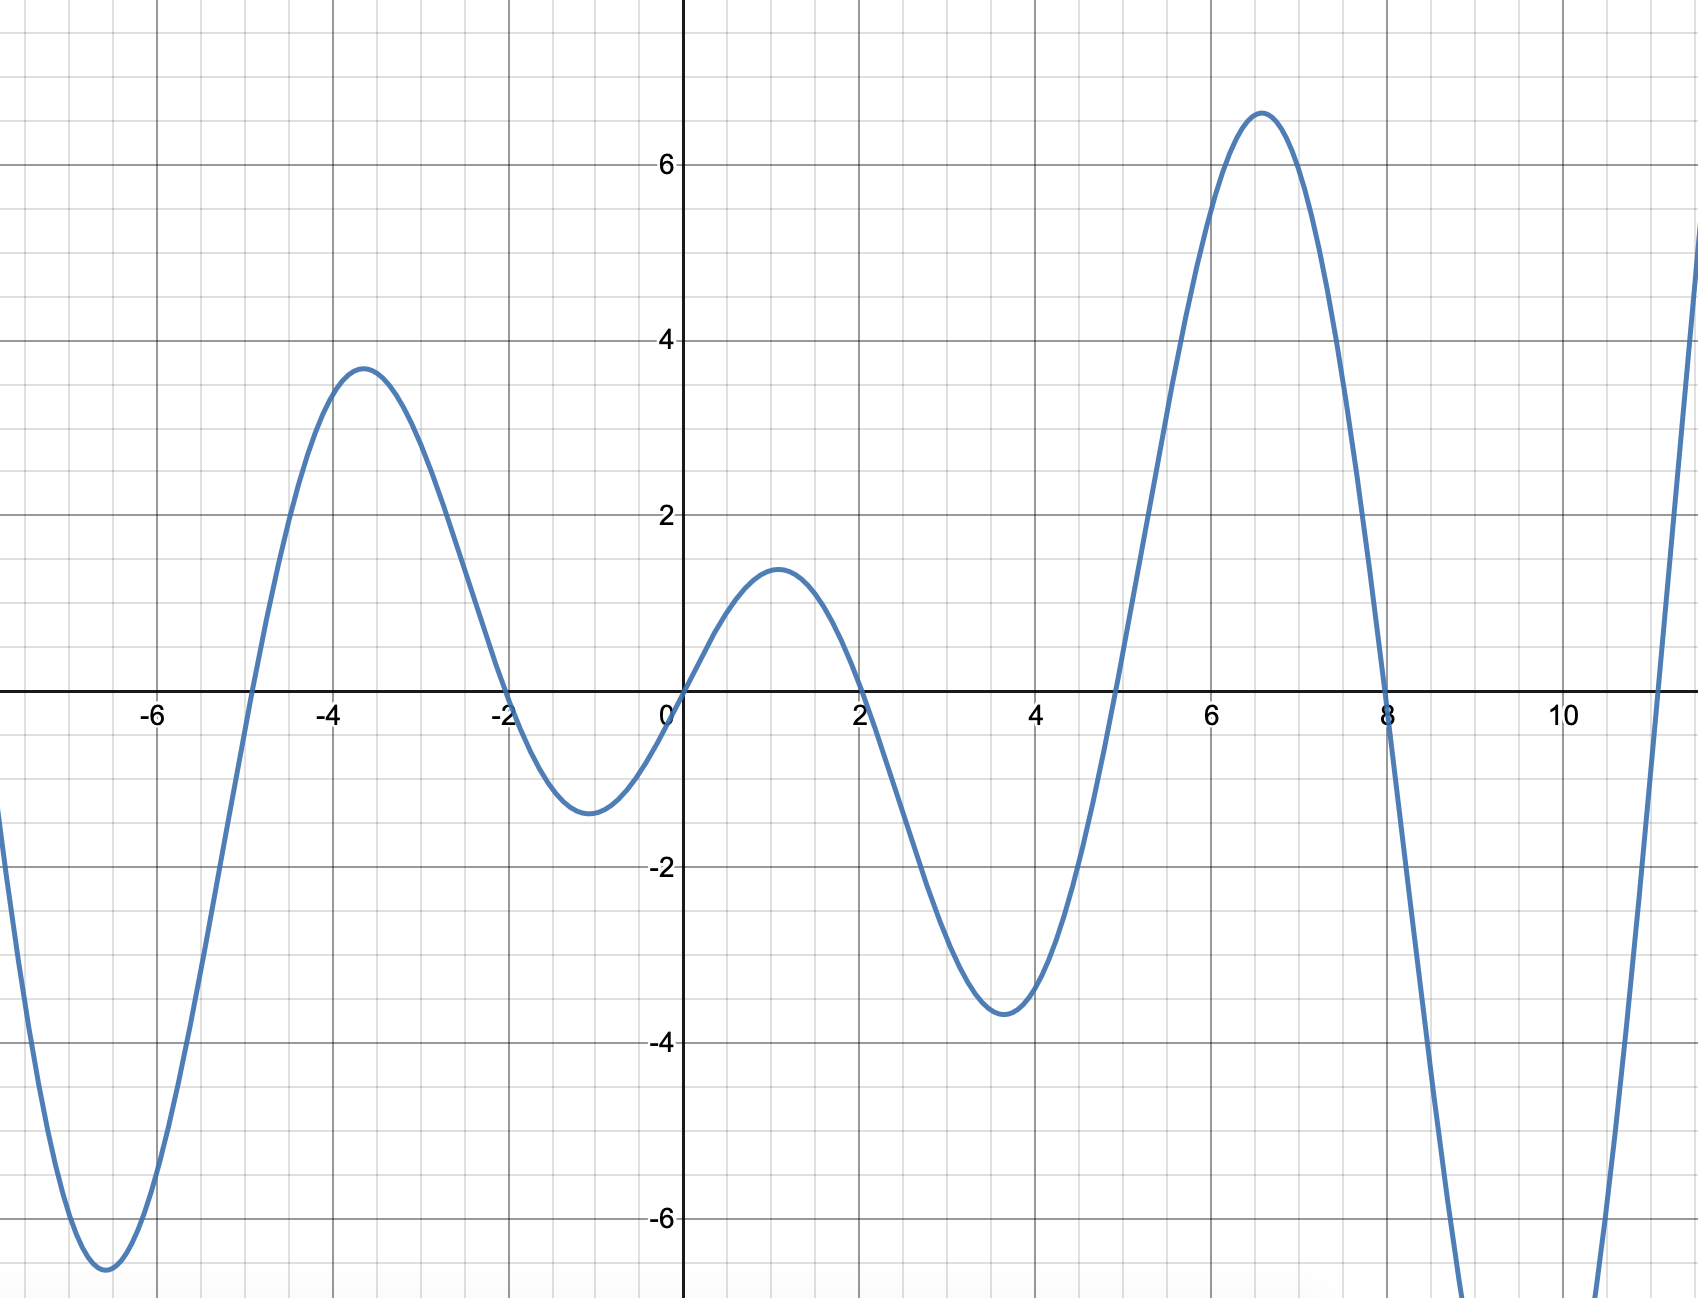
\includegraphics[scale=0.4]{lab5_32.png} \par
%     \vspace{2mm}
    
% \end{center}

% \hfil{Rysunek 4: Wykres funkcji $f(x) = e^{-x} - x$ w przybliżeniu} \par

\vspace{3mm}

W tym przypadku funkcja jest okresowa i ma nieskończenie wiele pierwiastków, dlatego dla przykładu policzymy dwa pierwsze z nich w przedziałach: $[0.5, 1.5]$ i  $[2.5, 3]$
\vspace{3mm}
Tak jak poprzednio sprawdzimy warunek $f(a) \cdot f(b)<0$ dla tych przedziałów: 

$$f(0.5) \cdot f(1.5) \approx-0.377287<0$$
$$f(2.5) \cdot f(3) \approx-0.286117<0$$

Warunek został spełniony dla obydwu przedziałów został spełniony więc dwa pierwsze przerwiastki tej funkcji na pewno znajdują się w tych przedziałach. Metodą Newtona-Raphson policzymy te pierwiastki. Najpierw musimy sprawdzić znak wyrażenia $f'(x)*f''(x)$ dla punktów brzegowych przedziałów: 

$$f^{\prime}(x)=x \cdot \cos (x)+\sin (x)$$
$$f^{\prime \prime}(x)=2 \cos (x)-x \cdot \sin (x)$$

\vspace{3mm}
$$f^{\prime}(0.5)=0.9182, f^{\prime \prime}(0.5)=1.5155$$
$$f^{\prime}(1.5)=1.1036, f^{\prime \prime}(1.5)=-1.3548 $$
\vspace{3mm}
$$f^{\prime}(2.5)=-1.4044, f^{\prime \prime}(2.5)=-3.0985$$
$$f^{\prime}(3)=-2.8289, f^{\prime \prime}(3)=-2.4034$$

\vspace{4mm}
W pierwszym przedziale znaki różnią się więc musmy sprawdzić warunek zbieżności dla obu wartości brzegowych: $x=0.5:\left|\frac{f(x) \cdot f^{\prime \prime}(x)}{\left(f^{\prime}(x)\right)^{2}}\right|<1 \Leftrightarrow\left|\frac{f(0.5) \cdot f^{\prime \prime}(0.5)}{\left(f^{\prime}(0.5)\right)^{2}}\right|<1 \Leftrightarrow 1.36656<1$ - sprzeczność, więc nie będziemy brać pod uwagę tego punktu. Sprawdźmy jeszcze warunek dla $x=1.5:\left|\frac{f(x) \cdot f^{\prime \prime}(x)}{\left(f^{\prime}(x)\right)^{2}}\right|<1 \Leftrightarrow\left|\frac{f(1.5) \cdot f^{\prime \prime}(1.5)}{\left(f^{\prime}(1.5)\right)^{2}}\right|<1 \Leftrightarrow 0.552<1$. Więc dla $x \in[0.5, 1.5]: x_{0}=a=0.5$
Ustalmy jeszcze warunek stopu - dobierając dokładność obliczeń równạ np. $\varepsilon=10^{-5}$.
\newline



$
\begin{array}{ll}
x_{0}=0.5 \\
x_{1}=0.5-\frac{f(0.5)}{f^{\prime}(0.5)} \approx 1.328 &
\left|x_{1}-x_{0}\right| \approx 0.828004 \\
x_{2}=1.328-\frac{f(1.328)}{f^{\prime}(1.328)} \approx 1.1039 &
\left|x_{2}-x_{1}\right| \approx 0.224083 \\
x_{3}=1.1039-\frac{f(1.1039)}{f^{\prime}(1.1039)} \approx 1.11415349 &
\left|x_{3}-x_{2}\right| \approx 0.0102322 \\
x_{4}=1.11415-\frac{f(1.11415)}{f^{\prime}(1.11415)} \approx 1.11415714 &
\left|x_{4}-x_{3}\right| \approx 3.65 \cdot 10^{-6}<\varepsilon
\end{array}
$
\vspace{3mm}
\newline
Dla $x_{4}$ warunek został spełniony. Zatem można uznać, że dla określonej dokładności $\varepsilon=10^{-5}$ wynik $x_{4} \approx 1.11415714$ jest szukanym miejscem zerowym funkcji.

\vspace{7mm}
Dla drugiego punktu wartość wyrażenia jest dodatnia więc dla $x \in[2.5, 3]: x_{0}=b=3$.


$
\begin{array}{ll}
x_{0}=3 \\ 
x_{1}=3-\frac{f(3)}{f^{\prime}(3)} \approx 2.796158 &
\left|x_{1}-x_{0}\right| \approx 0.203842 \\
x_{2}=2.7962-\frac{f(2.7962)}{f^{\prime}(2.7962)} \approx 2.77294969 &
\left|x_{2}-x_{1}\right| \approx 0.0232083 \\
x_{3}=2.77295-\frac{f(2.77295)}{f^{\prime}(2.77295)} \approx 2.77260478 &
\left|x_{3}-x_{2}\right| \approx 0.00034491 \\
x_{4}=2.7726-\frac{f(2.7726)}{f^{\prime}(2.7726)} \approx 2.77260471 &
\left|x_{4}-x_{3}\right| \approx 7 \cdot 10^{-8}<\varepsilon
\end{array}
$

\vspace{3mm}
Dla $x_{4}$ warunek został spełniony. Zatem można uznać, że dla określonej dokładności $\varepsilon=10^{-5}$ wynik $x_{4} \approx 2.77260471$ jest szukanym miejscem zerowym funkcji.

\vspace{6mm}
Ze względu na symetrię otrzymaliśmy miejsca zerowe: $x_{1}=\pm 1.11415714$ oraz $x_{2}=\pm 2.77260471$.


\section{Zapisz iteracje Newtona do rozwiązywania następującego układu równań nieliniowych.}
$$
x_1^2 + {x_2}^2 = 1 
$$ $$
x_1^2 - x_2 = 0
$$

W tym zadaniu korzystamy z Metody Newtona dla układu równań.
Metoda Newtona dla funkcji wielu zmiennych jest uogólnieniem tej metody dla funkcji jednej zmiennej. W metodzie stycznych wykorzystywaliśmy wzór: $f(x) \approx f\left(x_{0}\right)+f^{\prime}\left(x_{0}\right)\left(x-x_{0}\right)$ Jeżeli przyjąć, że $x \approx x_{0}$ to
$$
\text { otrzymywalismy: } f\left(x_{0}\right)+f^{\prime}\left(x_{0}\right)\left(x-x_{0}\right)=0 \Rightarrow x=x_{0}-\frac{f\left(x_{0}\right)}{f^{\prime}\left(x_{0}\right)} \text { . }
$$

Dla funkcji wielu zmiennych gdy $f=\left(f_{1}, f_{2}, \ldots, f_{n}\right): \mathbb{R}^{n} \rightarrow \mathbb{R}^{n}$ możemy f przybliżyć równaniem afi-
Jeśli założymy, że $x \approx x_{0}$ to:
$$
f\left(x_{0}\right)+D f\left(x_{0}\right)\left(x-x_{0}\right)=0 \Rightarrow f\left(x_{0}\right)+D f\left(x_{0}\right) x-D f\left(x_{0}\right) x_{0}=0 \Rightarrow D f\left(x_{0}\right) x=D f\left(x_{0}\right) x_{0}-f\left(x_{0}\right)
$$
Gdy $D f\left(x_{0}\right)$ jest odwracalna to: $x=\left[D f\left(x_{0}\right)\right]^{-1} D f\left(x_{0}\right)\left(x_{0}\right)-\left[D f\left(x_{0}\right)\right]^{-1} f\left(x_{0}\right)=I\left(x_{0}\right)-\left[D f\left(x_{0}\right)\right]^{-1} f\left(x_{0}\right)$.
A zatem ostatecznie $\quad x=\left(x_{0}\right)-\left[D f\left(x_{0}\right)\right]^{-1} f\left(x_{0}\right)$
Ogólnie można napisać: $f_{i}\left(x_{1}, x_{2}, \ldots, x_{n}\right)=0 \equiv F(X)=0, \quad$ gdzie $X=\left(x_{1}, x_{2}, \ldots, x_{n}\right), F=\left(f_{1}, f_{2}, \ldots, f_{n}\right)$
$$
\text { Zatem: } 0=F(X) \approx F\left(X_{0}\right)+D F\left(X_{0}\right)\left(X-X_{0}\right)
$$
A więc otrzymujemy rekurencyjne rozwiązanie: $X_{k+1}=X_{k}-\left[D F\left(X_{k}\right)\right]^{-1} F\left(X_{k}\right)$
Dla naszego zadania otrzymamy nastepujące równania:
$$
\begin{array}{c}
F(X)=\left[\begin{array}{l}
f_{1}(X) \\
f_{2}(X)
\end{array}\right]=\left[\begin{array}{l}
f_{1}(x, y) \\
f_{2}(x, y)
\end{array}\right]=\left[\begin{array}{c}
x^{2}+y^{2}-1 \\
x^{2}-y
\end{array}\right] \\
D F(X)=\left[\begin{array}{ll}
\frac{\partial f_{1}(x, y)}{\partial x} & \frac{\partial f_{1}(x, y)}{\partial y} \\
\frac{\partial_{2}(x, y)}{\partial x} & \frac{\partial_{2}(x, y)}{\partial y}
\end{array}\right]=\left[\begin{array}{cc}
2 x & 2 y \\
2 x & -1
\end{array}\right] \\
X_{k+1}=X_{k}-\left[\begin{array}{cc}
2 x & 2 y \\
2 x & -1
\end{array}\right]^{-1} \cdot\left[\begin{array}{c}
x^{2}+y^{2}-1 \\
x^{2}-y
\end{array}\right]
\end{array}
$$

Wykres poniżej przedstawia przebieg funkcji. Musimy w przybliżeniu określić granice przedzziału, w którym znajduje się dany pierwiastek.




\begin{center}
    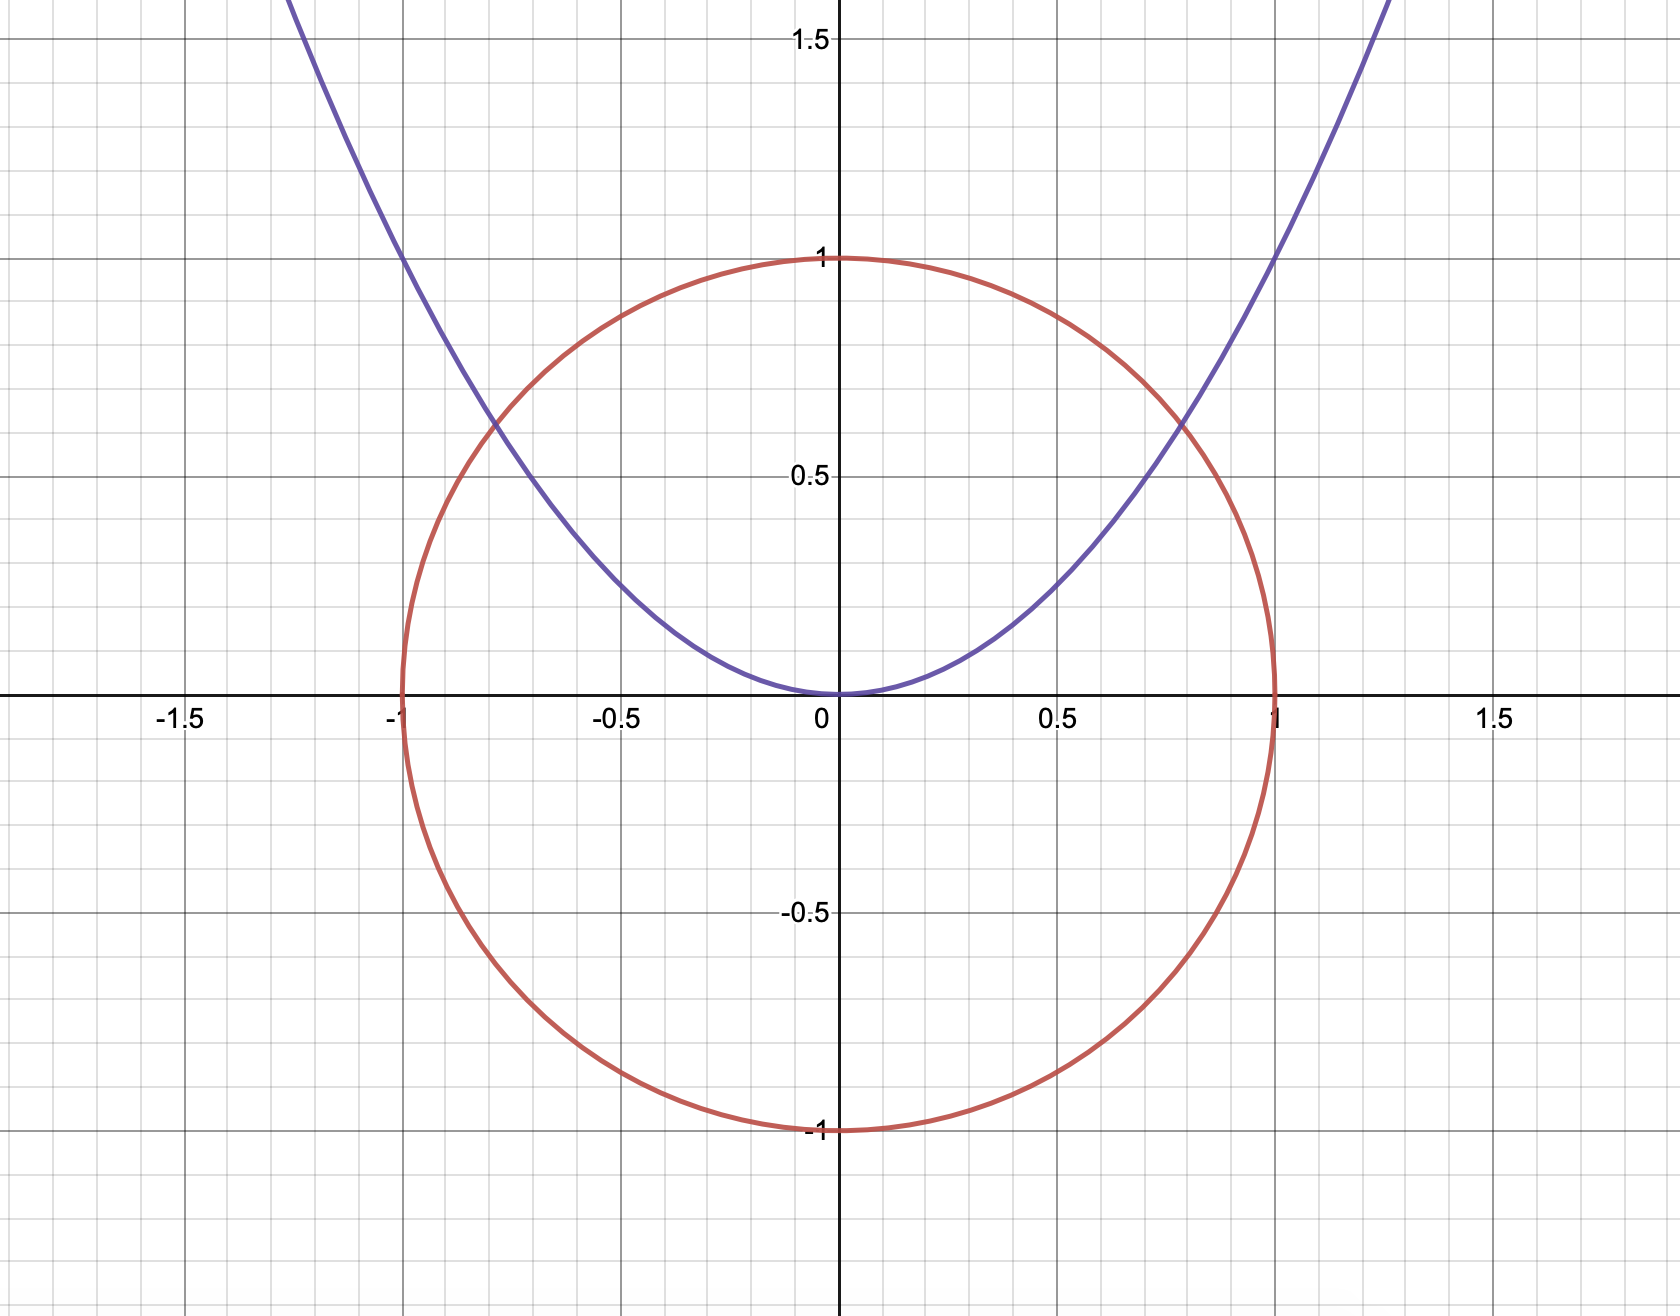
\includegraphics[scale=0.4]{lab5_4.png} \par
    \vspace{3mm}
    
\end{center}

\hfil{Rysunek 6} \par
\hfil{Czerowny: $x_1^2 + x_2^2 - 1 = 0$} \par
\hfil{Niebieski: $f(x) = x_1^2 - x_2$} \par

\vspace{5mm}

Z wykresu możemy wywnioskować, że pierwiastek będzie mieścił się w granicach $x \in[0.5 ; 1]$ oraz $x \in[-1 ;-0.5]$, a $y \in[0.5 ; 1]$. Ponieważ rozwiązanie $x$ jest symetryczne, rozwiążemy tylko jeden przypadek.

\vspace{3mm}

Wybieramy punkt startowy $\left(x_{0}, y_{0}\right)=(1,1)$. Obliczenia zostały wykonane za pomocą programu komputerowego:

$
\begin{array}{l}
$\left(x_{0}, y_{0}\right)=(1,1)$ \\
$\left(x_{1}, y_{1}\right)=(0.8(3) ; 0 .(6))$ \\
$\left(x_{2}, y_{2}\right)=(0.7881 ; 0.619)$ \\
$\left(x_{3}, y_{3}\right)=(0.78615407 ; 0.6180344)$ \\
$\left(x_{4}, y_{4}\right)=(0.78615138 ; 0.618034)$ \\
\end{array}
$

\vspace{4mm}


Otrzymujemy więc dwa rozwiązania (0.78615138; 0.618034) oraz (-0.78615138; 0.618034). Oczywiście powinniśmy ustalić warunek stopu, co pokazane zostało na przykładach w zadaniu 1). W tym zadaniu ograniczę się do warunku, którym jest ilość wykonanych iteracji równa w tym wypadku 4 .




\section{Bibliografia}

\begin{enumerate}
  \item \url{http://home.agh.edu.pl/~funika/mownit/lab5/wyklad_02.pdf}
  \item \url{http://wazniak.mimuw.edu.pl/index.php?title=MN02#Metoda_Newtona}
\end{enumerate}

\end{document}
